\documentclass[tikz]{standalone}

\usepackage{pgf, pgfplots}

\begin{document}
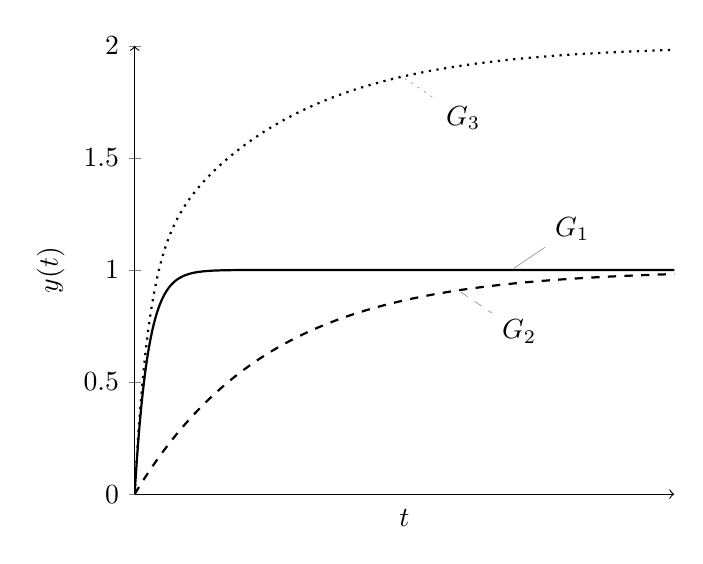
\begin{tikzpicture}
\begin{axis}[
axis lines=left,
axis line style={->},
xtick=\empty,
%ytick=\empty,
%xmin=-1,
%xmax=2,
%ymin=-1,
ymax=2,
xlabel=$t$,
ylabel=$y(t)$,
]
\addplot[solid,thick,domain=0:40, samples=400] {1-exp(-x)} node[pos=0.7, inner sep=0pt,pin=30:{$G_1$}] {};
\addplot[dashed,thick,domain=0:40, samples=400] {1-exp(-0.1*x)} node[pos=0.6, inner sep=0pt,pin=-30:{$G_2$}] {};
\addplot[dotted,thick,domain=0:40, samples=400] {2-exp(-0.1*x)-exp(-x) } node[pos=0.5, inner sep=0pt,pin=-30:{$G_3$}] {};
\end{axis}
\end{tikzpicture}
\end{document}
